%!TEX root = ../bachelorthesis.tex
\chapter{Grundlagen}
\label{chap:grundlagen}
Kameras sind viel genutzte Sensoren, da sie teilweise recht günstig hergestellt werden, und sie aufgrund ihrer Ähnlichkeit zum menschlichen Auge gute Sensoren sind, um die Umgebung zu erfassen. Da sich aber gezeigt hat, dass die Toleranzen bei der Produktion, der Aufbau der Kameras und insbesondere ihrer Linsen, zu Verzerrungen im Bild führen, wurden Modelle entwickelt, um diese Verzerrungen herauszurechnen und das Bild zu korrigieren. Ein häufig genutztes Modell wird im folgenden beschrieben.

\section{Kameramodell} % (fold)
\label{sec:kameramodell}
In \cite{Zhang} wird ein gängiges Kameramodell beschrieben, welches hier erklärt wird. Dieses Modell wird auch von OpenCV, siehe \cite{opencv}, und HALCON, siehe \cite{halcon} benutzt.

Die Beziehung zwischen einem Punkt $(u, v)$ in einem zweidimensionalen Bild und einem Punkt $(x, y, z)$ in der dreidimensionalen Welt wird durch \autoref{projection} beschrieben:

\begin{equation}
\begin{bmatrix}
 	u \\
 	v \\
 	1
\end{bmatrix} = K 
\begin{bmatrix}
   	R & T
\end{bmatrix} 
\begin{bmatrix}
   	x \\
   	y \\
   	z \\
   	1
\end{bmatrix} \label{projection}
\end{equation}

mit 

\begin{equation}
  K = 
  \begin{bmatrix}
  	f_x & 0 & c_x \\
  	0 & f_y & c_y \\
  	0 & 0 & 0
  \end{bmatrix}
\end{equation}

$K$ enthält die intrinsischen Parameter der Kamera, die auf Grund der Fertigungstoleranzen für jede Kamera unterschiedlich sind. $f$ definiert die Brennweite der Kamera. Da die Pixel nicht immer quadratisch sind, wird dieser Wert für die x und y-Achse angegeben. $c_x$ und $c_y$ beschreiben das optische Zentrum des Bildes, welches ebenfalls nicht immer genau im Mittelpunktes des Bildes liegt.

$R$ und $T$ definieren die extrinsischen Parameter. $R$ ist eine Rotationsmatrix, die die Rotation zwischen dem Kamera- und Weltkoordinatensystem beschreibt, $T$ ist ein Vektor, der die Transformation zwischen Kamera- und Weltkoordinatensystem beschreibt.

\section{Verzeichnung}
\label{sec:verzeichnung}
Mit dem Kameramodell kann nun eine Beziehung zwischen einem Punkt im Bild und dem Punkt in der Welt hergestellt werden. Kameras bilden das Bild jedoch nicht immer korrekt ab. Häufig erkennt man in Bildern den Effekt, dass gerade Linien in der Realität, wie z.B. Häuserkanten, nicht gerade im Bild abgebildet werden, sondern das diese gebogen sind. Diesen Effekt nennt man Verzeichnung.

Es gibt zwei verschiedene Formen von Verzeichnung. Ist die Verzeichnung radialsymmetrisch zum Bildmittelpunkt, spricht man von kissen- oder tonnenförmiger Verzeichnung, siehe \autoref{img:verzeichnung}.
\begin{figure}[!hbt]
	\centering
	\vspace{1ex}
	\includegraphics[scale=3]{../images/Verzeichnung}
	\caption[Beispiele für radialsymmetrische Verzeichnung, von Wikipedia: \cite{wiki:verzeichnung}]{\label{img:verzeichnung}Beispiele für radialsymmetrische Verzeichnung, von Wikipedia: \cite{wiki:verzeichnung}}
	\vspace{1ex}
\end{figure}

Die zweite Form von Verzeichnung beschreibt die tangentiale Verzeichnung. Siehe dazu \autoref{img:tangential_distortion}.
\begin{figure}[!hbt]
	\centering
	\vspace{1ex}
	\includegraphics[scale=0.5]{../images/tangential_distortion}
	\caption[Die durchgezogenen Linien sind ohne Verzeichnung, die gestrichelten Linien zeigen die tangentiale Verzeichnung. Aus: \cite{tangential_distortion}]{\label{img:tangential_distortion}Die durchgezogenen Linien sind ohne Verzeichnung, die gestrichelten Linien zeigen die tangentiale Verzeichnung. Aus: \cite{tangential_distortion}}
	\vspace{1ex}
\end{figure}

Es existieren verschiedene Modelle, um diese Verzeichnungen zu beschreiben. Das Divisionsmodell kann die radialsymmetrische Verzeichnung beschreiben und herausrechnen. Dazu wird nur ein einziger Parameter $k$ benötigt. Dies hat den Vorteil, dass nur relativ wenig Bilder benötigt werden, um einen guten Wert für $k$ zu erhalten. Der Nachteil an diesem Modell ist, dass nur die radialsymmetrische Verzeichnung erfasst wird und nicht die tangentiale Verzeichnung. Zudem ist die radialsymmetrische Verzeichnung nicht immer über das ganze Bild gleich verteilt, sodass das Modell nicht jede Situation optimal beschreibt.

Das Polynommodell kann hingegen beide Formen der Verzeichnung beschreiben. Dazu werden insgesamt fünf Parameter benötigt, welche im folgenden beschrieben werden. Die radialsymmetrische Verzeichnung kann in diesem Modell feiner bestimmt werden und die tangentiale Verzeichnung wird ebenfalls beachtet. Der Nachteil ist, dass mehr Bilder benötigt werden, um gute Ergebnisse zu erhalten. Außerdem ist es bei diesem Modell sehr wichtig, dass unterschiedliche Distanzen beachtet werden und das Muster in jedem Ausschnitt des Bildes zu sehen ist, da ansonsten die Werte für die nicht betrachteten Teile des Bildes extrem schlechte Ergebnisse liefern können.

Um die radialsymmetrische Verzeichnung herauszurechnen, werden die drei Faktoren $k_1, k_2, k_3$ benötigt. Sind diese gegeben, lässt sich die Verzeichnung mit den beiden folgenden Gleichungen korrigieren. $r$ ist der Abstand vom Bildmittelpunkt zu dem Punkt, der korrigiert werden soll. $x', y'$ sind die falsch abgebildeten Punkte, $x,y$ sind die korrigierten Punkte.
\begin{equation}
	x = x'(1 + k_1 r^2 + k_2 r^4 + k_3 r^6)
\end{equation}
\begin{equation}
	y = y'(1 + k_1 r^2 + k_2 r^4 + k_3 r^6)
\end{equation}

Um die tangentiale Verzeichnung zu korrigieren, werden die beiden folgenden Gleichungen benutzt. Dazu werden die Faktoren $p_1, p_2$ benötigt.
\begin{equation}
	x = x' + (2 p_1 xy + p_2 (r^2 + 2 x^2))
\end{equation}
\begin{equation}
	y = y' + (p_1(r^2 + 2 y^2) + 2p_2 xy)
\end{equation}

\section{Kalibrierung} % (fold)
\label{sec:kalibrierung}
Der Kalibrierungsvorgang dient dazu, die intrinsischen und gegebenenfalls extrinsischen Parameter sowie die Verzeichnungsparameter zu berechnen. Dies erfolgt in mehreren Schritten.

\subsection{Kalibrierungsmuster} % (fold)
\label{sub:kalibrierungsmuster}
Man benötigt ein Kalibrierungsmuster, von dem einige Aufnahmen gemacht werden. Es gibt verschiedene Kalibrierungsmuster, die benutzt werden können. Eine grundlegende gemeinsame Eigenschaft aller Kalibrierungsmuster ist, dass das Muster aus geometrischen Formen besteht, die gut von Bilderkennungsalgorithmen gefunden werden können. Häufig wird dazu ein Schachbrettmuster benutzt, siehe \autoref{img:chess5x7x0.03}. In diesem Muster haben die Rechtecke eine Kantenlänge von exakt 3cm. Inge samt sind 6 x 8 Rechtecke in dem Muster vorhanden. Der Kalibrierungsalgorithmus sucht nach den Kanten der Quadrate. Der Schnittpunkt von zwei Kanten, also die Ecke eines Quadrats, bildet den Kalibrierungspunkt. Dadurch enthält ein Bild mit diesem Kalibrierungsmuster 5 x 7, also 35, Kalibrierungspunkte.

\begin{figure}[!hbt]
	\centering
	\vspace{1ex}
	\includegraphics[scale=0.3, angle=90]{../images/chess5x7x3}
	\caption[Schachbrettmuster als Kalibrierungsmuster]{\label{img:chess5x7x0.03} Schachbrettmuster als Kalibrierungsmuster}
	\vspace{1ex}
\end{figure}

Ein anderes Kalibrierungsmuster besteht aus Kreisen, die regelmäßig versetzt zueinander positioniert sind, siehe \autoref{img:caltab_hex_10x11}. In diesem Muster sind die Mittelpunkte der Kreise die Kalibrierungspunkte. In diesem Muster sind 10 x 11 Kreise eingezeichnet, sodass deutlich mehr Informationen für die Kalibrierung in einer Aufnahme vorhanden sind. 

\begin{figure}[!hbt]
	\centering
	\vspace{1ex}
	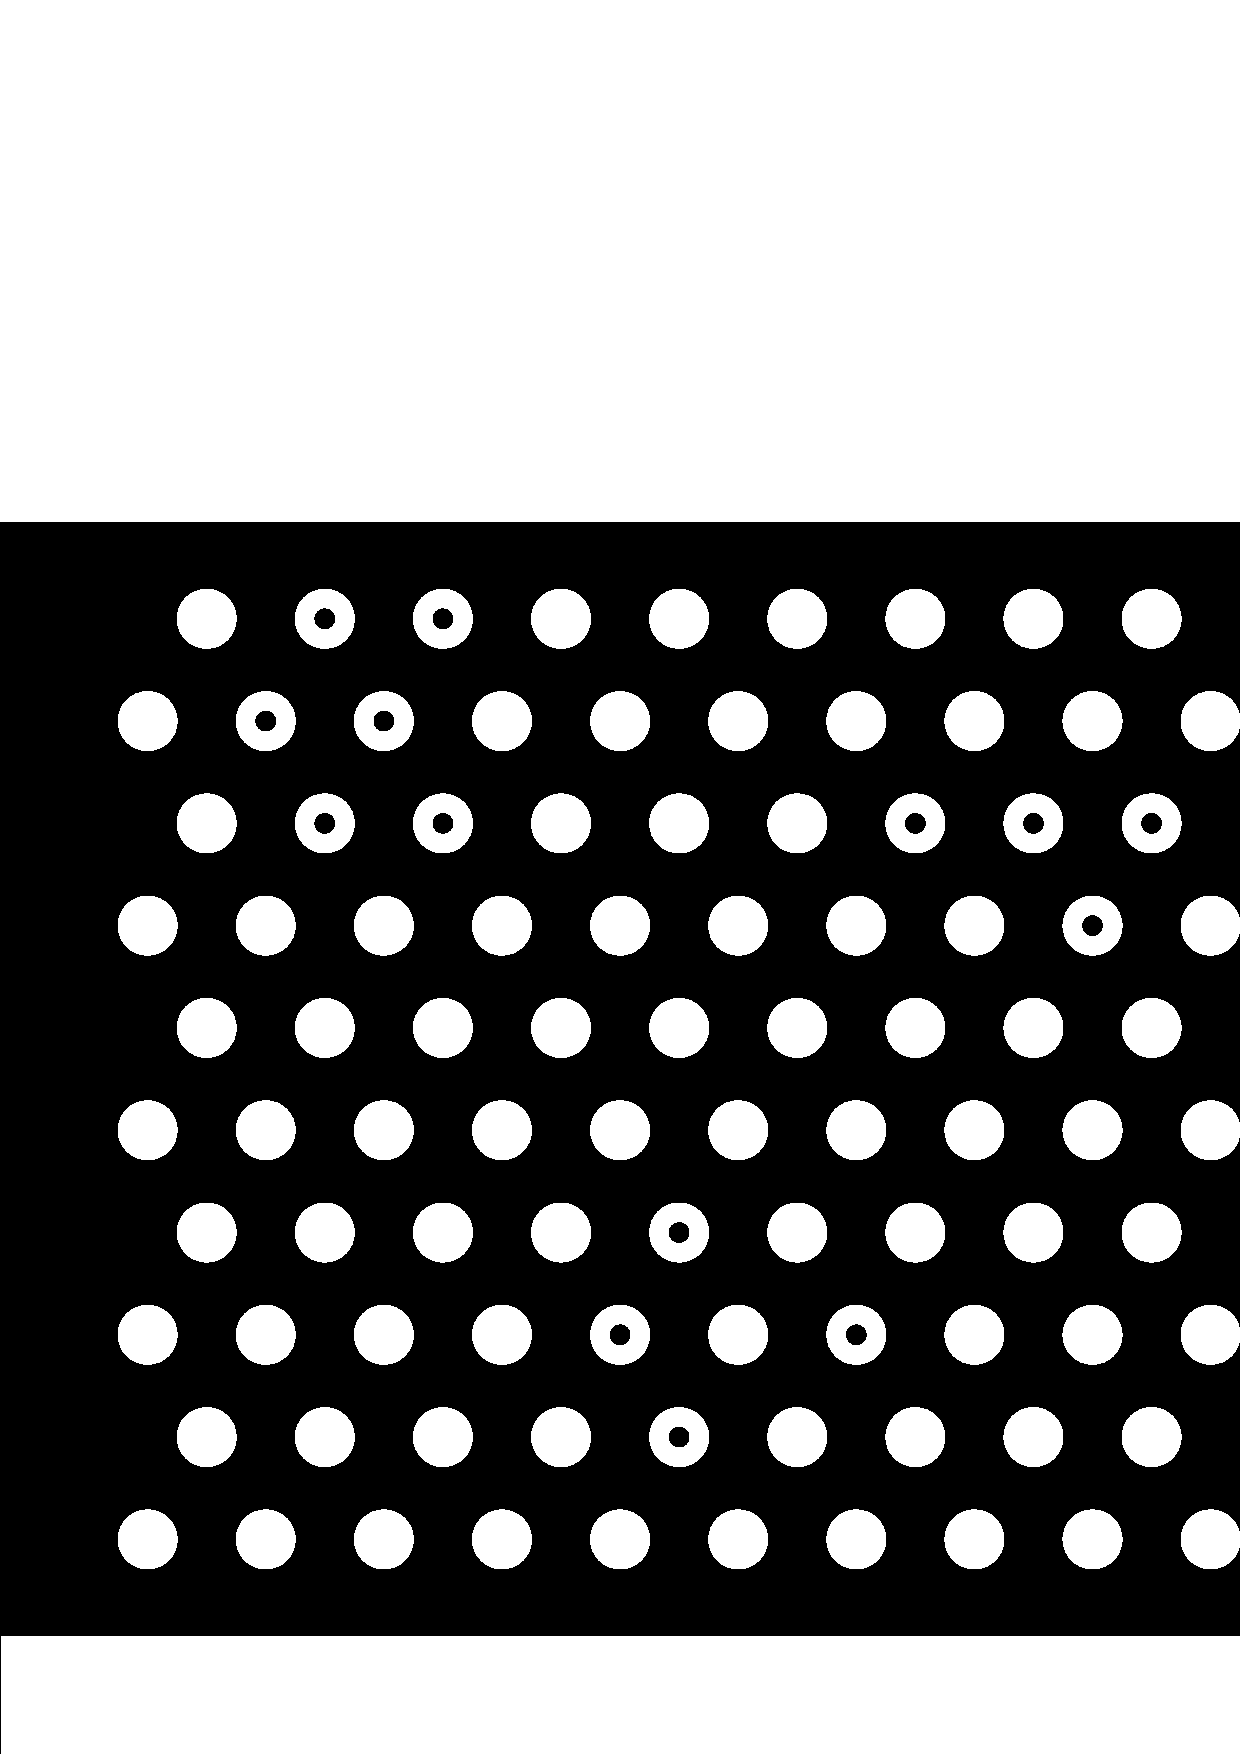
\includegraphics[scale=0.2]{../images/caltab_hex_10x11}
	\caption[Punkte als Kalibrierungsmuster]{\label{img:caltab_hex_10x11} Punkte als Kalibrierungsmuster}
	\vspace{1ex}
\end{figure}

Das Muster ist außerdem speziell für HALCON entwickelt. Während die Kreismuster von OpenCV im ganzen Bild den gleichen Punkt benutzen, sind in diesem Muster einzelne Punkte zusätzlich markiert. Dadurch kann HALCON auch dann noch Kalibrierungsinformationen aus einer Aufnahme errechnen, wenn das Kalibrierungsmuster nur teilweise zu sehen ist. Bei dem Schachbrettmuster oder dem Punktmuster von OpenCV muss hingegen immer das ganze Muster erkennbar sein.

Unabhängig davon, welches Muster man einsetzt, muss immer die Größe und Form der ausgedruckten Muster exakt den erwarteten Daten entsprechen. Da manche Drucker versuchen, die Dokumente auf DinA4-Größe anzupassen, muss man für jedes ausgedruckte Muster die Größe und Abstände der geometrischen Objekte überprüfen. Hat das ausgedruckte Muster die korrekte Größe, muss dieses auf eine möglichst ebene Oberfläche geklebt werden. Ein gekrümmtes Muster in einer Aufnahme, die zur Kalibrierung benutzt wird, kann die Ergebnisse verfälschen. Der Herstellen von HALCON, MVTec, bietet aus diesem Grund Kalibrierungsmuster zum Kauf an. Dies werden teilweise aus Aluminium hergestellt. MVTec garantiert dabei zum einen, dass die Abweichungen sehr gering sind, zum anderen können die Abweichungen exakt gemessen werden und der Kunde erhält zu dem Muster eine individuelle Datei, in der die exakten Abmessungen enthalten sind. Diese Datei kann dann zur Kalibrierung benutzt werden.

\subsection{Bildaufnahme} % (fold)
\label{sub:bildaufnahme}
Damit der Kalibrierungsalgorithmus die Parameter berechnen kann, muss er aus mehreren Bildern die Kalibrierungspunkte extrahieren. Dabei werden an die Bilder, die der Kalibrierung dienen, mehrere Anforderungen gestellt. 

Wie bei anderen Fotos auch, ist es wichtig, dass das Motiv, also das Kalibrierungsmuster, scharf dargestellt wird und gut belichtet ist. Dabei ist es hilfreich, wenn Kamera und Kalibrierungsmuster auf Stativen befestigt sind. 

Wenn das Polynommodell zur Beschreibung der Verzeichnung benutzt wird, besteht eine erhöhte Gefahr der Überanpassung. Überanpassung beschreibt das Problem, wenn die gefundenen Parameter zwar sehr gut auf die Situation passen, die zur Kalibrierung untersucht wurde, aber in anderen Situationen sehr schlechte Ergebnisse liefern. In diesem Kontext muss man daher darauf achten, dass das Muster in verschiedenen Distanzen zur Kamera aufgenommen wurde. Ansonsten können die Parameter schlechte Ergebnisse erzeugen, wenn Objekte betrachtet werden, die deutlich näher oder weiter entfernt von der Kamera sind als das Muster.

Ist das Muster nur an einer Stelle im Bild zu sehen und an anderen Stellen gar nicht, kann ebenfalls eine Überanpassung auftreten. Daher muss das Muster über alle Aufnahmen verteilt im ganzen Bild sichtbar sein. 

Die Kalibrierung wird zusätzlich verbessert, wenn das Muster nicht immer orthogonal zur Kamera steht sondern auch horizontal oder vertikal geneigt wird.

\subsection{Berechnung der Parameter} % (fold)
\label{sub:berechnung_der_parameter}
Wurden genügend Bilder aufgenommen, die den Anforderungen entsprechen, können die Parameter berechnet werden. Dazu ist eine initiale Konfiguration der intrinsischen Parameter nötig. Die dafür notwendigen Informationen kann man den Spezifikationen der Kamera oder des Sensors entnehmen. Die Brennweite $f$ wird in der Regel vom Hersteller angegeben. Für das optische Zentrum $c_x$ und $c_y$ kann man die Bildmitte, also die halbe Auflösung des Bildes, annehmen.

Anschließend werden in jedem aufgenommenen Bild die Kalibrierungspunkte extrahiert und abgespeichert. Im nächsten Schritt werden dann mit diesen Informationen die Gleichungssysteme gelöst, die die gesuchten Parameter enthalten. Zusätzlich zu den Parametern berechnen die Algorithmen den durchschnittlichen Fehler in Pixeln. Dieser sollte möglichst klein, am besten unter eins, sein. Wird das Kalibrierungsmuster nicht in verschiedenen Orientierungen aufgenommen oder es ist nicht im ganzen Bildausschnitt zu sehen, kann dies den Fehler vergrößern.

Es gibt mehrere Frameworks, die man zum Kalibrieren benutzen kann. OpenCV ist eine freie Bibliothek zur Bildverarbeitung und zum maschinellen Sehen. Es wird kein fertiges Programm angeboten, mit dem der Vorgang direkt gestartet werden kann. Stattdessen existieren Bibliotheken in C++ und Python, in denen der Benutzer Funktionen findet, mit denen er sein eigenes Programm schreiben kann, um eine Kamera zu kalibrieren. Für Benutzer, die mit dieser Materie nicht so vertraut sind, ist dies eine hohe Hürde. Profis können damit aber das Programm auf die eigenen Bedürfnisse anpassen.

Ein anderes Framework ist HALCON. Es wird kommerziell vermarktet und ist nicht frei verfügbar. Wie bei OpenCV werden Bibliotheken für verschiedene Programmiersprachen angeboten, mit denen Benutzer ihre eigenen Programme schreiben können. Zusätzlich existiert mit HDevelop eine integrierte Entwicklungsumgebung. In HDevelop wird eine eigene Programmiersprache benutzt, die weniger tief und detailliert als andere Sprachen ist, aber dafür für unerfahrene Benutzer deutlich sprechender und intuitiver zu benutzen ist. Außerdem ist ein Kalibrierungsassistent enthalten, der die aufgenommen Bilder vor der Berechnung der Parameter anhand ihrer Bildschärfe, Belichtung und weiterer Eigenschaften bewertet. Des Weiteren ist es von Vorteil, dass HALCON nicht das ganze Muster sehen muss, sondern bereits Teile davon zur Kalibrierung benutzt werden können. Teilweise haben die Algorithmen eine geringere Laufzeit. In der Arbeitsgruppe Künstliche Intelligenz von Prof. Beetz wird HALCON intensiv eingesetzt.

\subsection{Weitere benutzte Frameworks} % (fold)
\label{sub:weitere_benutzte_frameworks}
\subsubsection{ROS} % (fold)
\label{ssub:ros}
ROS \cite{ROS} steht für Robot Operating System. Es wurde entwickelt, um ein Framework für die Programmierung von unterschiedlichen Robotern zur Verfügung zu stellen. Möglich ist die Einbindung fertiger Pakete, die von anderen Benutzern bereitgestellt werden, zum Beispiel MoveIt!, siehe\autoref{ssub:moveit}. Außerdem kann man kann außerdem eigene Programme schreiben und in ROS integrieren. ROS wird nicht nur für so einfache Roboter wir der UR5-Arm benutzt, sondern auch für komplexere Roboter wie der PR2 oder auch in autonom fahrenden Autos.

In der Regel startet man mehrere Programme, die jeweils eine bestimmte Aufgabe erfüllen sollen. Es gibt unterschiedliche Möglichkeiten, mit denen die Programme untereinander kommunizieren können. ROS stellt Bibliotheken für viele verschiedene Programmiersprachen bereit, damit man eigene Pakete schreiben kann, die sich in das Gesamtsystem integrieren lassen.

Im weiteren Verlauf werden einige ROS-spezifische Begrifflichkeiten benutzt, die nun kurz erklärt werden.

Da ein in ROS eingesetztes Programm einem bestimmten Zweck dient, werden meistens mehrere Programme parallel gestartet, die miteinander kommunizieren. Ein einzelnes Programm wird als \texttt{Node} bezeichnet. Die einzelnen Nodes bilden dazu ein eigenes kleines Netzwerk. Manche Nodes sprechen einen Sensor an, um seine Daten zu veröffentlichen und anderen Programmen zugänglich zu machen. Dazu veröffentlichen sie die Sensordaten auf einem \texttt{Topic}. Die Node, die die Daten veröffentlicht, nennt man dann \texttt{Publisher}. Die Nodes, die diese Daten empfangen möchten, um sie auszuwerten, nennt man \texttt{Subscriber}. 

Zusätzlich dazu gibt es die Möglichkeit, dass sich eine Node als \texttt{Actionserver} im Netzwerk registriert und andere Nodes als \texttt{Actionclients} Aufgaben an diese Node schicken können. Die Clients bekommen Informationen dazu, was für eine Aufgabe ein Actionserver anbietet und welche Parameter der Client angeben kann. Erhält der Server eine Aufgabe, versucht er sie durchzuführen und gibt dem Client zurück, ob die Aufgabe erfolgreich ausgeführt wurde oder nicht. Anschließend wartet der Actionserver auf weitere Aufgaben.

Benutzer können interne Parameter einer Node zum Startzeitpunkt ändern, wenn der Programmierer dies vorgesehen hat. Dazu definiert der Benutzer beim Aufruf der Node \texttt{Argumente}, die an das Programm übergeben werden. Dadurch lässt sich zum Beispiel der Name eines Topics ändern, wenn man eine andere Kamera einsetzt. 

\subsubsection{MoveIt!} % (fold)
\label{ssub:moveit}
MoveIt! \cite{MoveIt} ist ein Framework, dass die Steuerung eines Roboters abstrahiert. MoveIt! stellt Bibliotheken für verschiedene Programmiersprachen bereit, mit denen man die Bewegung des Roboters kontrollieren kann. Möchte man wie in diesem Projekt einen Roboterarm steuern, kann man eine Zielposition und Orientierung für die Spitze des Arms angeben. MoveIt! berechnet für diese Kombination aus Position und Orientierung dann die Konfiguration der Robotergelenke. Im nächsten Schritt wird dann eine Abfolge von Zwischenkonfigurationen gesucht, damit sich der Roboter von seiner Startkonfiguration zur Zielkonfiguration bewegt, ohne dass er sich selbst oder andere Objekte in seiner Umgebung berührt. Existiert eine solche Abfolge von Konfigurationen, wird diese ausgeführt, sodass sich der Roboterarm letztendlich an der gewünschten Position mit der gewünschten Orientierung befindet.

\subsubsection{UR5} % (fold)
\label{ssub:ur5}
Der UR5 ist ein Roboterarm von Universal Robots. Dieser ist in drei verschiedenen Größen erhältlich, der UR5 ist die mittlere Größe. Alle UR-Roboter können kollaborierend mit Menschen arbeiten, sie müssen also nicht räumlich getrennt von Menschen arbeiten. Darüber hinaus lassen sie sich mit dem angeschlossenen Touchpad relativ einfach steuern und programmieren. Mit einem Knopf am Touchpad kann man den Roboter durch einfaches Bewegen des Arms an die gewünschte Position bringen und diese als Wegpunkt oder Position abspeichern. 

Zusätzlich wurde als ROS-Paket ein Interface geschrieben, um den Roboter auch über ROS und MoveIt! steuern zu können.
% subsubsection ur5 (end)